\begin{figure}[t]
  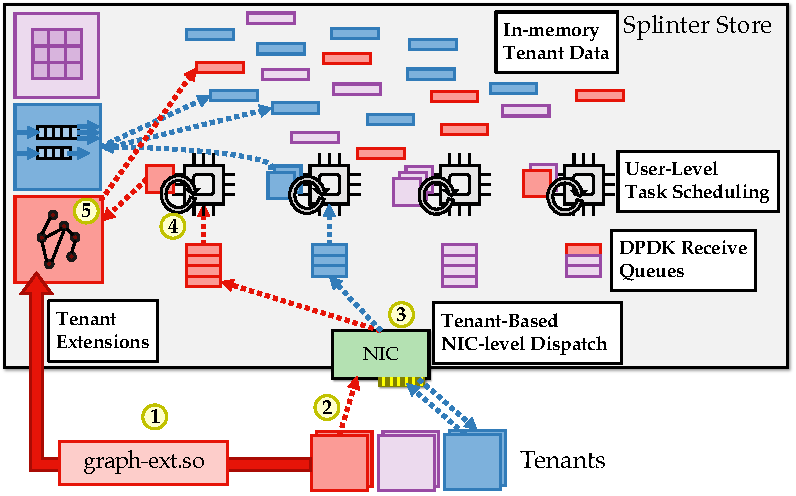
\includegraphics[width=1.0\columnwidth]{figures/splinter-arch.pdf}
  \caption{Overview of Splinter. Tenant data is stored in
  memory, and tenants can invoke extensions they have installed in the store (\textcircled{\footnotesize{1}}).
  Extensions are type safe, but compile to native code. The NIC uses
  kernel bypass for low latency (\textcircled{\footnotesize{2}}) and assists in dispatch by routing tenant
  requests to cores (\textcircled{\footnotesize{3}}). Each core runs
  a single {\sl worker} kernel thread that uses a user-level task scheduler to interleave
  the execution of tenant requests (\textcircled{\footnotesize{4}}).}
  \label{fig:arch}
\end{figure}
